\subsection{From Physics to Digital Signal Processing}

\begin{frame}[t]{Acoustic Impulse Response}

    \begin{block}{Sound interacts with environment}
        \begin{itemize}
            \item[] it is reflected (specularly and diffusely)\hspace{1em}\tikzmark{rightA}\tikzmark{topA}
            \item[$+$] it is diffracted
            \item[$+$] it is absorbers and transmitted
            \item[$+$] other physical interaction\tikzmark{botA}
        \end{itemize}
    \end{block}

    \vfill
    \only<1>{\textbf{Sound propagation} process = \textbf{source $\to$ filter $\to$ receiver} process
    \begin{equation*}
        x(t) = (a \ast s)(t)
    \end{equation*}
    The filter $a(t)$ is linear and is called \textbf{Acoustic Impulse Response}, (AIR)
    }
    \only<2->{\textbf{\alert{Indoor} Sound propagation} process = \textbf{source $\to$ filter $\to$ receiver} process
    \begin{equation*}
        x(t) = (h \ast s)(t)
    \end{equation*}
    The filter $h(t)$ is linear and is called \textbf{\alert{Room} Impulse Response}, (RIR)
    }

    \visible<2->{
        \vspace{5mm}
        \begin{columns}[T,onlytextwidth]
            \begin{column}{0.48\textwidth}
                \centering
                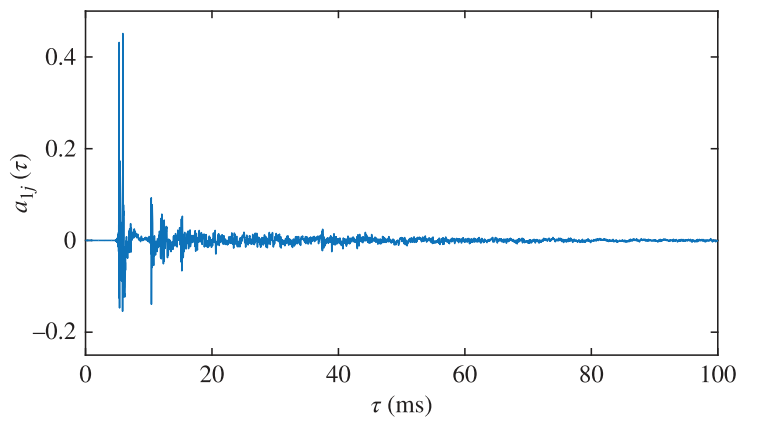
\includegraphics[width=\textwidth]{figures/rir_measured.png}
            \end{column}
            \begin{column}{0.48\textwidth}
                \centering
                \includegraphics<2>[width=\textwidth]{figures/rir_bang.png}
                \includegraphics<3->[width=\textwidth]{figures/rir_schematic.png}
            \end{column}
        \end{columns}
    }

    \begin{tikzpicture}[overlay, remember picture]
        \node[anchor=base] (a) at (pic cs:topA) {\vphantom{h}}; % push the mark to the top of the line (ie including ascenders)
        \node[anchor=base] (b) at (pic cs:botA) {\vphantom{g}}; % push the mark to the bottom of the line (ie including descenders)
        \draw [decoration={brace,amplitude=0.5em},decorate,thick,gray]
            (a.north -| {pic cs:rightA}) -- node[right,inner sep=1em]
                {$=$ all sound propagation}
            (b.south -| {pic cs:rightA});
    \end{tikzpicture}

    \begin{textblock*}{40mm}(90mm,47mm)
        \small \textcolor{gray}{$\leftarrow$ continuous time domain!}
    \end{textblock*}

    \only<4>{
        \begin{textblock*}{30mm}(62mm,72mm)
            \Large\textcolor{myred}{$\mathbf{\overset{?}{\approx}$}}
        \end{textblock*}

        \begin{textblock*}{40mm}(45mm,92mm)
            \centering
            \textcolor{myred}{!we observe filters, not delays}
        \end{textblock*}
    }

\end{frame}

\begin{frame}{Echoes and Room Impulse Response}

    \begin{columns}[onlytextwidth]
        \begin{column}{0.60\textwidth}
            \begin{block}{RIRs can be modeled with the Image Methods}
                \begin{itemize}
                    \item specular reflection only
                    \item = sound propagation of cuboid room
                    \item \textbf{well model the first part}
                \end{itemize}
            \end{block}
        \end{column}
        \begin{column}{0.38\textwidth}
            \centering
            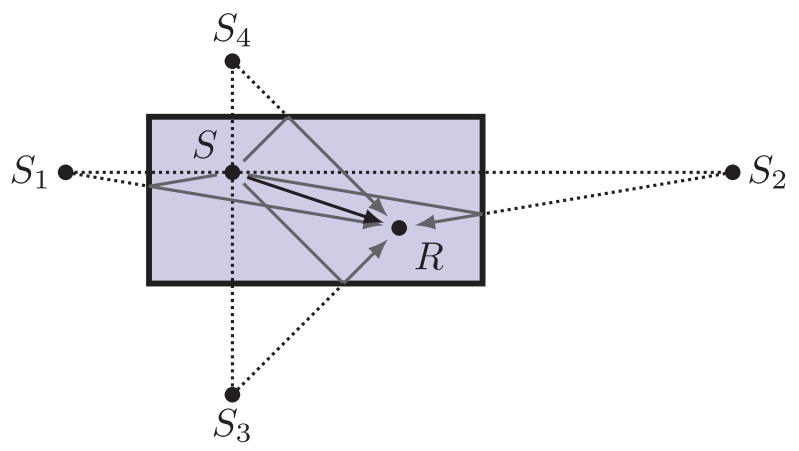
\includegraphics[width=\textwidth]{figures/ism.png}
            {\small ``playing billiard in a concert hall''}
        \end{column}
    \end{columns}

    \vfill
    \begin{columns}[onlytextwidth]
        \begin{column}{0.48\textwidth}
            \centering
            \textbf{Time domain}
            \begin{equation*}
                h^e(t) = \sum_r
            \end{equation*}
        \end{column}
        \begin{column}{0.48\textwidth}
            \centering
            \textbf{Frequency domain}
            \begin{equation*}
                H^e(f) = \sum_r
            \end{equation*}
        \end{column}
    \end{columns}

    \vfill
    \begin{block}{RIRs accounts for}

        \vspace{3mm}
        \begin{columns}[T,onlytextwidth]
            \column{0.48\textwidth}
            the \textbf{geometry} of the room
            \begin{itemize}
                \item \alert{Room shape and size}
                \item \alert{Mic and Source position}
                \item other objects (eg. reflectors)
            \end{itemize}
            \column{0.48\textwidth}
            the \textbf{acoustic properties} of
            \begin{itemize}
                \item surface materials
                \item objects materials
            \end{itemize}
        \end{columns}
    \end{block}

    \begin{center}
        \alert{Echoes} strong and distinct specular reflection as well
    \end{center}

\end{frame}

% \begin{frame}{Echoes in (Digital) Signal Processing}

%     \begin{block}{Room Impulse Response}
%         \begin{equation*}
%             \tilde{x}_i = (\tilde{h}_i \ast \tilde{s})(t) \longrightarrow \tilde{X}_i( f) = \tilde{H}_{ij}( f) \tilde{S}( f)
%         \end{equation*}
%         the linear filtering effect due to the propagation of sound from a source to a microphone in a indoor space
%     \end{block}

%     \begin{block}{Observation}
%         Our vision is limited both in time (finite and discrete) and in frequency (finite and discrete)
%         \begin{equation}
%             x_i[n] = ...
%         \end{equation}
%     \end{block}

%     \begin{block}{Signal model in the frequency domain}
%         \begin{equation*}
%             x_i = (h_i \ast s)(t)\;\longrightarrow\;X(f) = H_i(f) S(f)
%         \end{equation*}
%     \end{block}

%     \begin{block}{Approximations}
%         \begin{itemize}
%             \item Narrowband Approximation
%             \item DTFT echo model in the DFT
%         \end{itemize}
%     \end{block}

% \end{frame}

% \subsection*{interim conclusion}
% \begin{frame}{Interim Conclusion I}
%     \begin{alertblock}{Approximations}
%         \begin{itemize}
%             \item Echoes are well described by specular reflection
%             \item Echoes are off-grid by nature
%             \item Sampling and quantization make them hard
%             \item Processing in the discrete frequency domain, but with continuous time echo model
%         \end{itemize}
%     \end{alertblock}
% \end{frame}
